ORB-SLAM [1] is a feature-based (ORB features\footnote{ORB are binary features, invariant to rotation and scale (in a certain range), resulting in a very fast recognizer with good invariance to viewpoint})monocular simultaneous localization and mapping (SLAM) algorithm that operates in real time, in small/ large indoor and outdoor environments. ORB are oriented multi-scale FAST corners with a 256-bit descriptor associated. They are extremely fast to compute and match, while they have good invariance to viewpoint. This allows matching them with wide baselines, boosting the accuracy of bundle adjustment, BA. [2] presents the good performance of ORB for place recognition.

\begin{figure}[H]
	\centering
	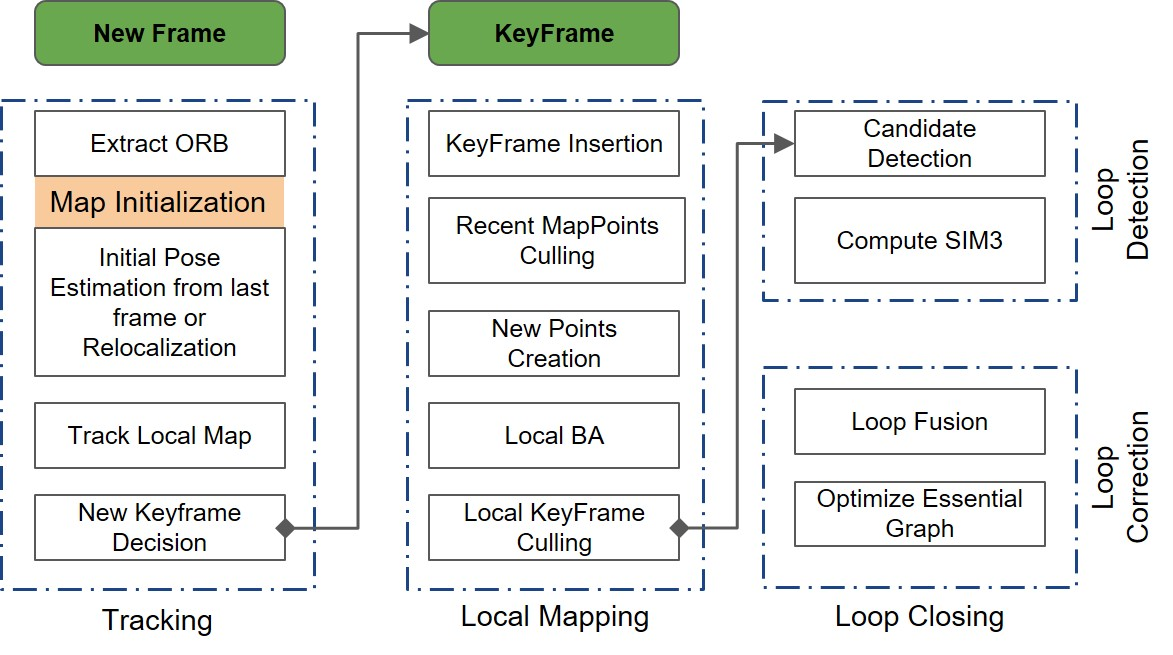
\includegraphics[width=1.0\linewidth]{figures/orb_slam_pipeline}
	\caption{Pipeline of the ORB SLAM algorithm}
	\label{fig:orbslampipeline}
\end{figure}

The main features of ORB-SLAM, are as described below:

a) ORB Features [3]: allow real-time operation without using GPUs. Additionally, it makes it possible to use the same features for all tasks including: tracking, mapping, re-localization, and loop closing.

b) Real-time operation: By using covisibility graph, tracking and mapping are focused in a local covisible area, independent of global map size.

c)Essential Graph: Real-time loop closing based on the optimization of a pose graph.

d)Real-time camera relocalization: Allows recovery from tracking failure and also enhances map reuse.

e)Initialization Procedure: using model selection permits creating initial map of planar and non-planar scenes.

f)Survival of the fittest approach to map point and keyframe selection that is generous in the spawning but very restrictive in the culling. This policy improves tracking robustness and enhances lifelong operation because redundant keyframes are discarded.
\\


The system is comprised of 3 parallel threads, shown in Fig. \ref{fig:orbslampipeline}:

\subsubsection{Tracking} 
A constant velocity motion model is assumed to predict the camera pose and perform guided search of the map points observed in the last frame. Optimization is performed over found correspondences. If tracking is lost, then the frame is converted into bag of words and re-localization is done by finding keyframe candidates from query to the recognition database. Once, estimation of the camera pose is done and an initial set of feature matches, the map can be projected into the frame and more map point correspondences can be searched (Refer to [1] for more details). As there is a mechanism in the local mapping to cull redundant keyframes, the algorithm tries to insert keyframes as fast as possible. This makes the tracking more robust to challenging camera movements, typically rotations. To insert a new keyframe, all the following conditions must be met[1]:

 a) More than 20 frames must have passed from the last global relocalization.


 b) Local mapping is idle, or more than 20 frames have passed from last keyframe insertion.


 c) Current frame tracks at least 50 points.


 d) Current frame tracks less than 90\% points than $K_{ref}$ (reference keyframe $K_{ref} \in K1 $, which shares most map points with current frame)
\\
\subsubsection{Local Mapping} 
with every new keyframe $K_i$, the covisibility graph is updated, adding a new node for $K_i$ and updating the edges resulting from the shared map points with other keyframes. Then the spanning tree is updated linking $K_i$ with the keyframe having most points in common. This is followed by computing the bags of words representation for the keyframe, which will help in the data association for triangulating new points. For a new map point to be retained it must fulfill these two conditions: First, the tracking must find the point in more than the 25\% of frames in which it is predicted to be visible. Second, if more than one keyframe have passed from map point creation, it must be observed from at least three keyframes. Once a map point have passed this test, it can only be removed if at any time it is observed from less than three keyframes. This can happen when keyframes are culled and when local BA discards outlier observations. This policy makes the map contain very few outliers.

\subsubsection{Loop Closing} 
To accept a loop candidate,  three consecutive consistent (keyframes connected in the co-visibility graph) loop candidates should be detected. Similarity transformation is calculated, from the current keyframe $K_i$ to the loop keyframe $K_l$, that represents the error accumulated in the loop. If similarity $S_{il}$ with  enough inliers is found, the loop with $K_l$ is accepted. After this loop fusion is done followed by Essential Graph Optimization.

%[image - ]